\chapter{Mammalian Tissues}\label{mammalian-tissues}

In biology,
\href{https://en.wikipedia.org/wiki/Tissue_(biology)}{tissue} is a
cellular organizational level between cells and a complete organ. A
tissue is an ensemble of similar cells and their extracellular matrix
from the same origin that together carry out a specific function. Organs
are then formed by the functional grouping together of multiple tissues.
The English word is derived from the French tissu, meaning something
that is woven, from the verb tisser, ``to weave''.

The study of human and animal tissues is known as histology or, in
connection with disease, histopathology. For plants, the discipline is
called plant anatomy. The classical tools for studying tissues are the
paraffin block in which tissue is embedded and then sectioned, the
histological stain, and the optical microscope. In the last couple of
decades, developments in electron microscopy, immunofluorescence, and
the use of frozen tissue sections have enhanced the detail that can be
observed in tissues. With these tools, the classical appearances of
tissues can be examined in health and disease, enabling considerable
refinement of medical diagnosis and prognosis.

\section{Animal tissues}\label{animal-tissues}

Animal tissues are grouped into four basic types: connective, muscle,
nervous, and epithelial. Collections of tissues joined in structural
units to serve a common function compose organs. While all animals can
generally be considered to contain the four tissue types, the
manifestation of these tissues can differ depending on the type of
organism. For example, the origin of the cells comprising a particular
tissue type may differ developmentally for different classifications of
animals.

\section{\texorpdfstring{\href{https://en.wikipedia.org/wiki/Connective_tissue}{Connective
tissue}}{Connective tissue}}\label{connective-tissue}

Connective tissues are made up of cells separated by non-living
material, which is called an extracellular matrix. This matrix can be
liquid or rigid. For example, blood contains plasma as its matrix and
bone's matrix is rigid. Connective tissue gives shape to organs and
holds them in place. Blood, bone, tendon, ligament, adipose and areolar
tissues are examples of connective tissues.

\section{\texorpdfstring{\href{https://en.wikipedia.org/wiki/Muscle_tissue}{Muscle
tissue}}{Muscle tissue}}\label{muscle-tissue}

Muscle cells form the active contractile tissue of the body known as
muscle tissue or muscular tissue. Muscle tissue functions to produce
force and cause motion, either locomotion or movement within internal
organs. Muscle tissue is separated into three distinct categories:
visceral or smooth muscle, found in the inner linings of organs;
skeletal muscle, typically attached to bones and which generates gross
movement; and cardiac muscle, found in the heart where it contracts to
pump blood throughout an organism.

\section{\texorpdfstring{\href{https://en.wikipedia.org/wiki/Nervous_tissue}{Nervous
tissue}}{Nervous tissue}}\label{nervous-tissue}

Cells comprising the central nervous system and peripheral nervous
system are classified as nervous (or neural) tissue. In the central
nervous system, neural tissues form the brain and spinal cord. In the
peripheral nervous system, neural tissues form the cranial nerves and
spinal nerves, inclusive of the motor neurons.

\section{\texorpdfstring{\href{https://en.wikipedia.org/wiki/Epithelium}{Epithelial
tissue}}{Epithelial tissue}}\label{epithelial-tissue}

The epithelial tissues are formed by cells that cover the organ surfaces
such as the surface of skin, the airways, the reproductive tract, and
the inner lining of the digestive tract. The cells comprising an
epithelial layer are linked via semi-permeable, tight junctions; hence,
this tissue provides a barrier between the external environment and the
organ it covers. In addition to this protective function, epithelial
tissue may also be specialized to function in secretion, excretion and
absorption. Epithelial tissue helps to protect organs from
microorganisms, injury, and fluid loss.

Functions of epithelial tissue:

\begin{itemize}
\tightlist
\item
  The cells of the body's surface form the outer layer of skin.
\item
  Inside the body, epithelial cells form the lining of the mouth and
  alimentary canal and protect these organs.
\item
  Epithelial tissues help in absorption of water and nutrients.
\item
  Epithelial tissues help in elimination of waste.
\item
  Epithelial tissues secrete enzymes and/or hormones in the form of
  glands.
\end{itemize}

There are many kinds of epithelium, and nomenclature is somewhat
variable. Most classification schemes combine a description of the
cell-shape in the upper layer of the epithelium with a word denoting the
number of layers: either simple (one layer of cells) or stratified
(multiple layers of cells). However, other cellular features, such as
cilia may also be described in the classification system.

Some common kinds of epithelium are listed below:

\begin{itemize}
\tightlist
\item
  Simple squamous epithelium
\item
  Stratified squamous epithelium
\item
  Simple cuboidal epithelium
\item
  Transitional epithelium
\item
  Pseudostratified columnar epithelium (also known as Ciliated columnar
  epithelium)
\item
  Columnar epithelium
\item
  Glandular epithelium
\item
  Ciliated columnar epithelium
\end{itemize}

\begin{figure}

{\centering 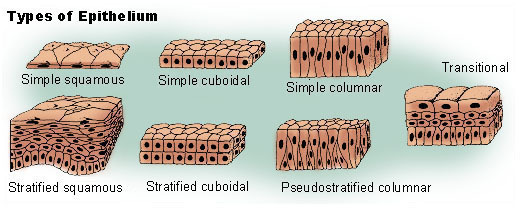
\includegraphics[width=0.7\linewidth]{./figures/tissues/epithelium}

}

\caption{\href{https://commons.wikimedia.org/wiki/File:Illu_epithelium.jpg}{Types
of epithelia}}\label{fig:epithelium}
\end{figure}

\section{Animal Organs}\label{animal-organs}

In biology, an organ or viscus is a collection of tissues joined in a
structural unit to serve a common function. In anatomy, a viscus is an
internal organ, and viscera is the plural form.

Organs are composed of main tissue, parenchyma, and ``sporadic''
tissues, stroma. The main tissue is that which is unique for the
specific organ, such as the myocardium, the main tissue of the heart,
while sporadic tissues include the nerves, blood vessels, and connective
tissues. The main tissues that make up an organ tend to have common
embryologic origins, such as arising from the same germ layer.
Functionally related organs often cooperate to form whole organ systems.
Organs exist in all higher biological organisms, in particular they are
not restricted to animals, but can also be identified in plants. In
single-cell organisms like bacteria, the functional analogue of an organ
is called organelle.

A hollow organ is a visceral organ that forms a hollow tube or pouch,
such as the stomach, intestine, or bladder.

\section{Animal Organ Systems}\label{animal-organ-systems}

Two or more organs working together in the execution of a specific body
function form an organ system. The functions of organ systems often
share significant overlap. For instance, the nervous and endocrine
system both operate via a shared organ, the hypothalamus. For this
reason, the two systems are combined and studied as the neuroendocrine
system. The same is true for the musculoskeletal system because of the
relationship between the muscular and skeletal systems.

Mammals such as humans have a variety of organ systems. These specific
systems are also widely studied in human anatomy.

\begin{itemize}
\tightlist
\item
  \href{https://en.wikipedia.org/wiki/Circulatory_system}{Cardiovascular
  system}: pumping and channeling blood to and from the body and lungs
  with heart, blood and blood vessels.
\item
  \href{https://en.wikipedia.org/wiki/Human_digestive_system}{Digestive
  system}: digestion and processing food with salivary glands,
  esophagus, stomach, liver, gallbladder, pancreas, intestines, colon,
  rectum and anus.
\item
  \href{https://en.wikipedia.org/wiki/Endocrine_system}{Endocrine
  system}: communication within the body using hormones made by
  endocrine glands such as the hypothalamus, pituitary gland, pineal
  body or pineal gland, thyroid, parathyroids and adrenals, i.e.,
  adrenal glands.
\item
  \href{https://en.wikipedia.org/wiki/Excretory_system}{Excretory
  system}: kidneys, ureters, bladder and urethra involved in fluid
  balance, electrolyte balance and excretion of urine.
\item
  \href{https://en.wikipedia.org/wiki/Lymphatic_system}{Lymphatic
  system}: structures involved in the transfer of lymph between tissues
  and the blood stream, the lymph and the nodes and vessels that
  transport it including the Immune system: defending against
  disease-causing agents with leukocytes, tonsils, adenoids, thymus and
  spleen.
\item
  \href{https://en.wikipedia.org/wiki/Integumentary_system}{Integumentary
  system}: skin, hair and nails.
\item
  \href{https://en.wikipedia.org/wiki/Muscular_system}{Muscular system}:
  movement with muscles.
\item
  \href{https://en.wikipedia.org/wiki/Nervous_system}{Nervous system}:
  collecting, transferring and processing information with brain, spinal
  cord and nerves.
\item
  \href{https://en.wikipedia.org/wiki/Reproductive_system}{Reproductive
  system}: the sex organs, such as ovaries, fallopian tubes, uterus,
  vulva, vagina, testes, vas deferens, seminal vesicles, prostate and
  penis.
\item
  \href{https://en.wikipedia.org/wiki/Respiratory_system}{Respiratory
  system}: the organs used for breathing, the pharynx, larynx, trachea,
  bronchi, lungs and diaphragm.
\item
  \href{https://en.wikipedia.org/wiki/Skeleton}{Skeletal system}:
  structural support and protection with bones, cartilage, ligaments and
  tendons.
\end{itemize}

\section{View Prepared Slides of
Tissues}\label{view-prepared-slides-of-tissues}

\begin{enumerate}
\def\labelenumi{\arabic{enumi}.}
\tightlist
\item
  Lung simple squamous epithelium (Figure \ref{fig:lung})

  \begin{itemize}
  \tightlist
  \item
    Identify flattened cells with noticeable nucleus.
  \end{itemize}
\item
  Stratified squamous epithelium (Figure \ref{fig:stratifiedsquamous})

  \begin{itemize}
  \tightlist
  \item
    Identify: layers of squamous epithelium cells, with a greater
    concentration of living, nucleate cells towards the side of contact
    with the rest of the tissues.
  \end{itemize}
\item
  Simple cuboidal epithelium (Figure \ref{fig:cuboidal})

  \begin{itemize}
  \tightlist
  \item
    Identify: cuboidal shaped cells with large, central nucleus. Notice
    the attachment end versus the end facing the open space.
  \end{itemize}
\item
  Simple columnar epithelium (Figure \ref{fig:columnar})

  \begin{itemize}
  \tightlist
  \item
    Identify: rectangular shaped cells with nucleus at the base, goblet
    cells with mucus, cilia, and basement membrane.
  \end{itemize}
\item
  Amphibian stratified ciliated columnar epithelium

  \begin{itemize}
  \tightlist
  \item
    Identify: ciliated columnar epithelial cells
  \end{itemize}
\item
  Pseudostratified ciliated columnar epithelium (Figure
  \ref{fig:pseudociliated})

  \begin{itemize}
  \tightlist
  \item
    Identify: pseudostratification, position of nuclei, goblet cells
    filled with mucus, and cilia
  \end{itemize}
\item
  Areolar tissue spread (Figure \ref{fig:areolar})

  \begin{itemize}
  \tightlist
  \item
    Identify: fibroblasts, collagen fibers, elastic fibers.
  \end{itemize}
\item
  Dense fibrous irregular

  \begin{itemize}
  \tightlist
  \item
    Identify: fibroblasts' nuclei, collagen bundles
  \end{itemize}
\item
  White fibrous tissue human (Figure \ref{fig:whitefibrous})

  \begin{itemize}
  \tightlist
  \item
    Identify: fibroblasts' nuclei, collagen bundles
  \end{itemize}
\item
  Adipose tissue (Figure \ref{fig:adipose})

  \begin{itemize}
  \tightlist
  \item
    Identify: fibroblasts filled with fat, nucleus, cell membrane,
    intercellular matrix
  \end{itemize}
\item
  Mammal hyaline cartilage (Figure \ref{fig:hyaline})

  \begin{itemize}
  \tightlist
  \item
    Identify: chondrocytes, lacunae, homogeneous matrix, perichondrium.
  \end{itemize}
\item
  Trachea monkey (Figure \ref{fig:trachea})

  \begin{itemize}
  \tightlist
  \item
    Identify: chondrocytes, lacunae, homogeneous matrix, perichondrium.
  \end{itemize}
\item
  Elastic cartilage human (Figure \ref{fig:elastic})

  \begin{itemize}
  \tightlist
  \item
    Identify: chondrocytes, lacunae, elastic fibers, perichondrium.
  \end{itemize}
\item
  Fibrocartilage (Figure \ref{fig:fibro})

  \begin{itemize}
  \tightlist
  \item
    Identify: chondrocytes, lacunae, collagen fibers
  \end{itemize}
\item
  Bone ground human (Figure \ref{fig:groundbone})

  \begin{itemize}
  \tightlist
  \item
    Identify: Haversian Systems, osteocytes in lacunae, Haversian Canal,
    canaliculi, calcified matrix
  \end{itemize}
\item
  Human blood Wright's smear (Figure \ref{fig:bloodsmear})

  \begin{itemize}
  \tightlist
  \item
    Identify: erythrocytes (red blood cells) - notice the approximately
    round shape, and the lack of nucleus -; leukocytes (white blood
    cells) - up to 5 different types, with nuclei in various shapes-;
    and the platelets (very small pieces of cells in the matrix).
  \end{itemize}
\item
  Sickle cell anemia (Figure \ref{fig:sickle})
\item
  Human skeletal muscle (Figure \ref{fig:skeletal})

  \begin{itemize}
  \tightlist
  \item
    Identify: each individual muscle fiber, nuclei, and striations.
  \end{itemize}
\item
  Cardiac muscle human

  \begin{itemize}
  \tightlist
  \item
    Identify: individual cells with one nucleus per cell, striations,
    intercalated disks, and branched muscle fibers.
  \end{itemize}
\item
  Cardiac muscle mammal (Figure \ref{fig:cardiac})

  \begin{itemize}
  \tightlist
  \item
    Identify: individual cells with one nucleus per cell, striations,
    intercalated disks, and branched muscle fibers.
  \end{itemize}
\item
  Smooth muscle mammal (Figure \ref{fig:smooth})

  \begin{itemize}
  \tightlist
  \item
    Identify: individual cells with one nucleus per cell, homogeneous
    cytoplasm, shape, and arrangement of the muscle fibers.
  \end{itemize}
\item
  Amphibian amooth muscle teased (Figure \ref{fig:teased})

  \begin{itemize}
  \tightlist
  \item
    Identify: individual smooth muscle cells with nucleus.
  \end{itemize}
\item
  Motor neuron smear (Figure \ref{fig:neuron})

  \begin{itemize}
  \tightlist
  \item
    Identify: cell body of neuron with nucleus, dendrites, axons (if
    possible), and neuroglial cells
  \end{itemize}
\end{enumerate}

\begin{figure}

{\centering 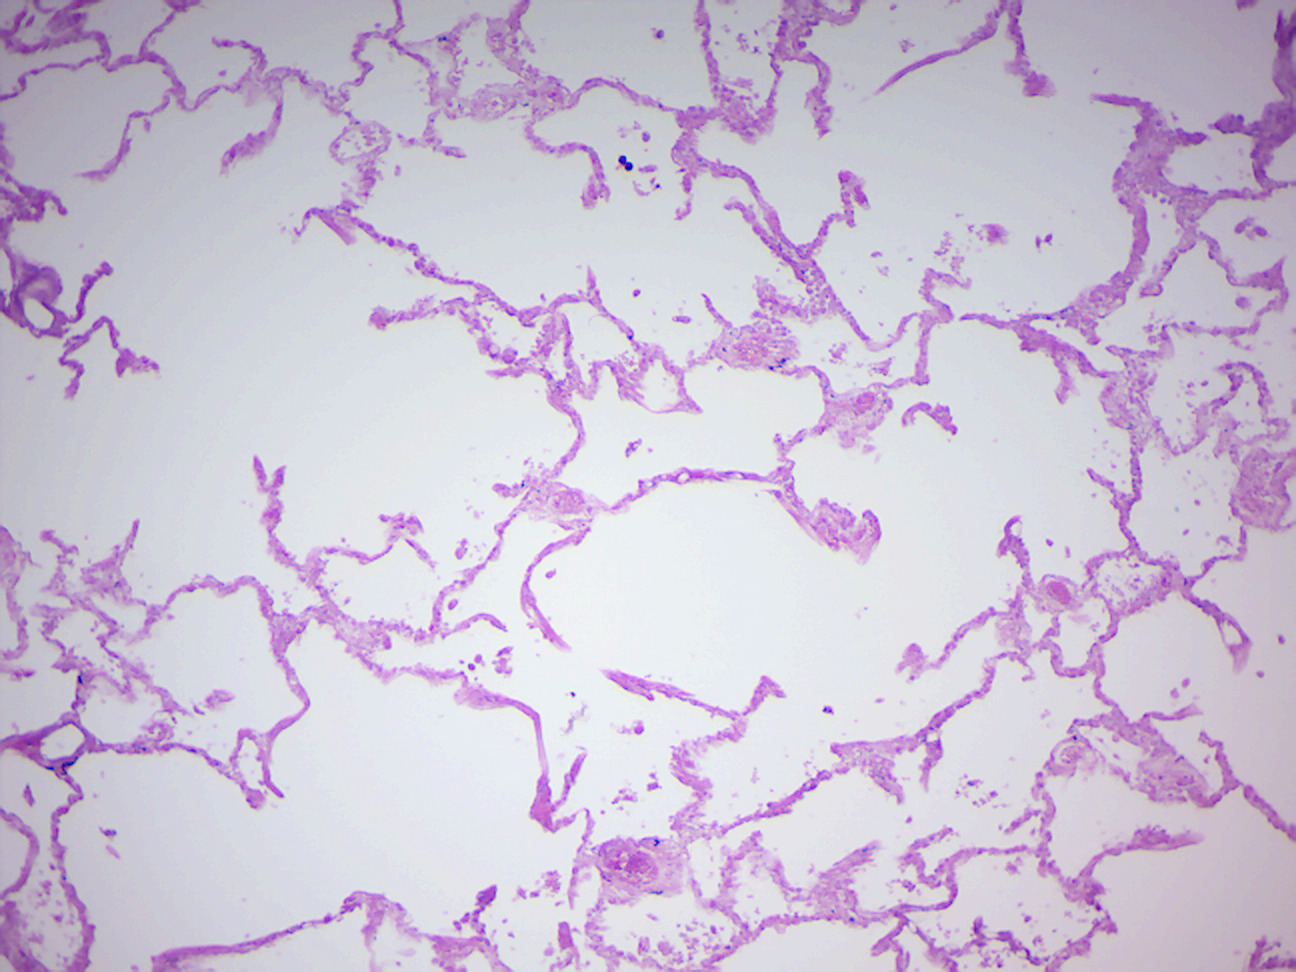
\includegraphics[width=0.7\linewidth]{./figures/tissues/lung_simple_squamous}

}

\caption{Simple squamous epithelium (human lung).}\label{fig:lung}
\end{figure}

\begin{figure}

{\centering 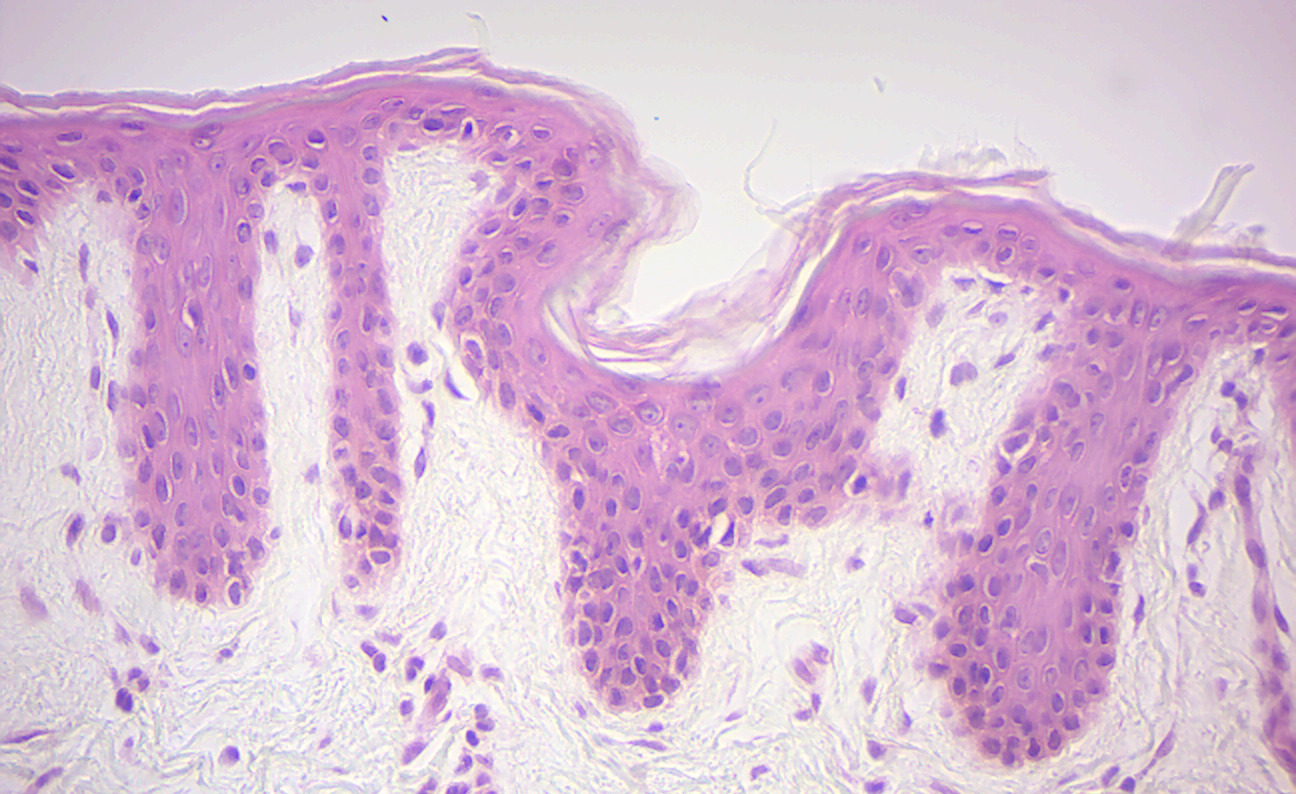
\includegraphics[width=0.7\linewidth]{./figures/tissues/stratified_squamous}

}

\caption{Stratified squamous epithelium (human epidermis).}\label{fig:stratifiedsquamous}
\end{figure}

\begin{figure}

{\centering 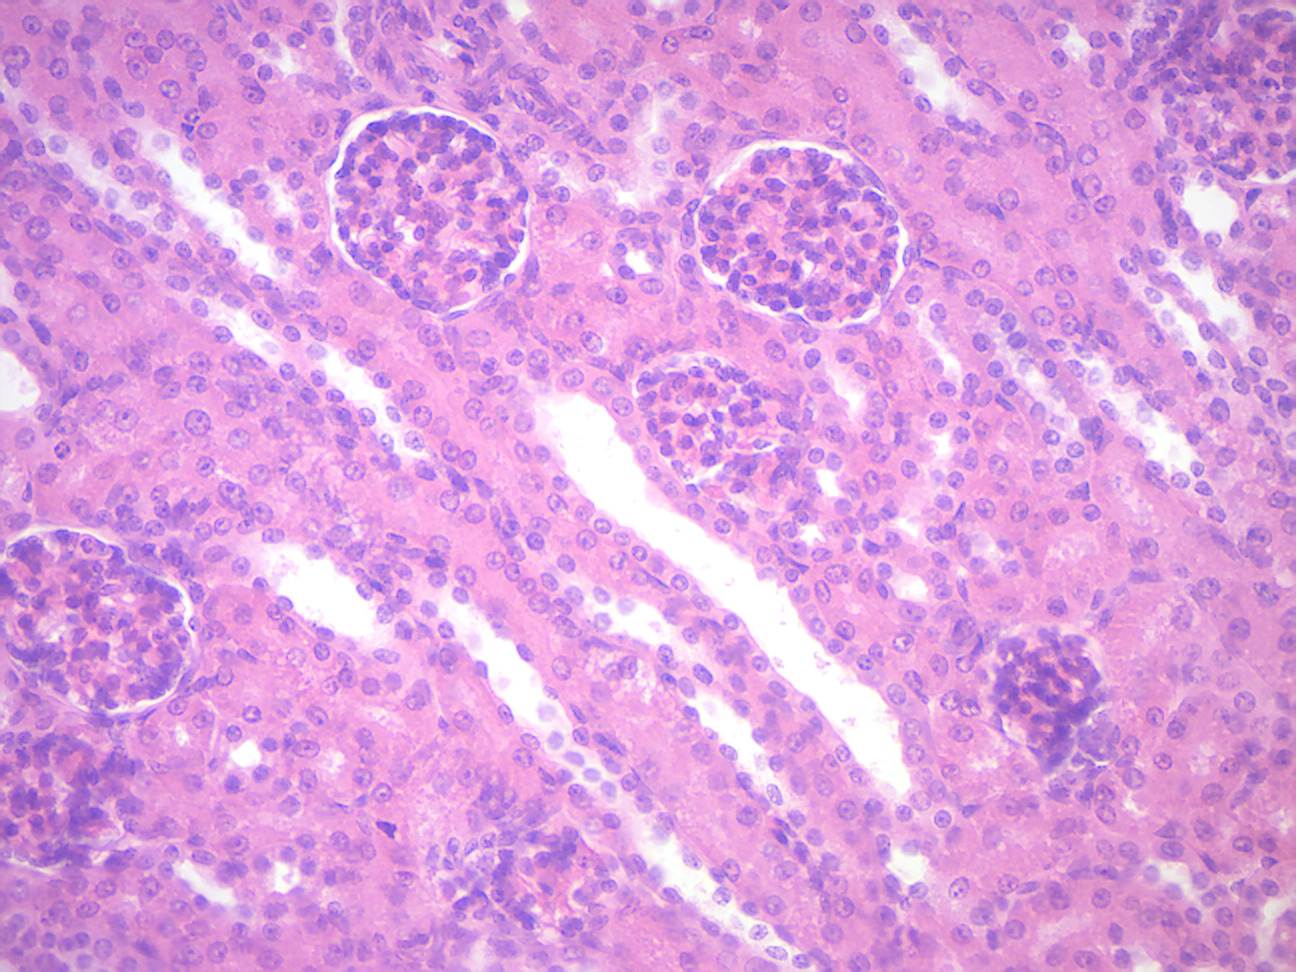
\includegraphics[width=0.7\linewidth]{./figures/tissues/simple_cuboidal}

}

\caption{Simple cuboidal epithelium (kidney).}\label{fig:cuboidal}
\end{figure}

\begin{figure}

{\centering 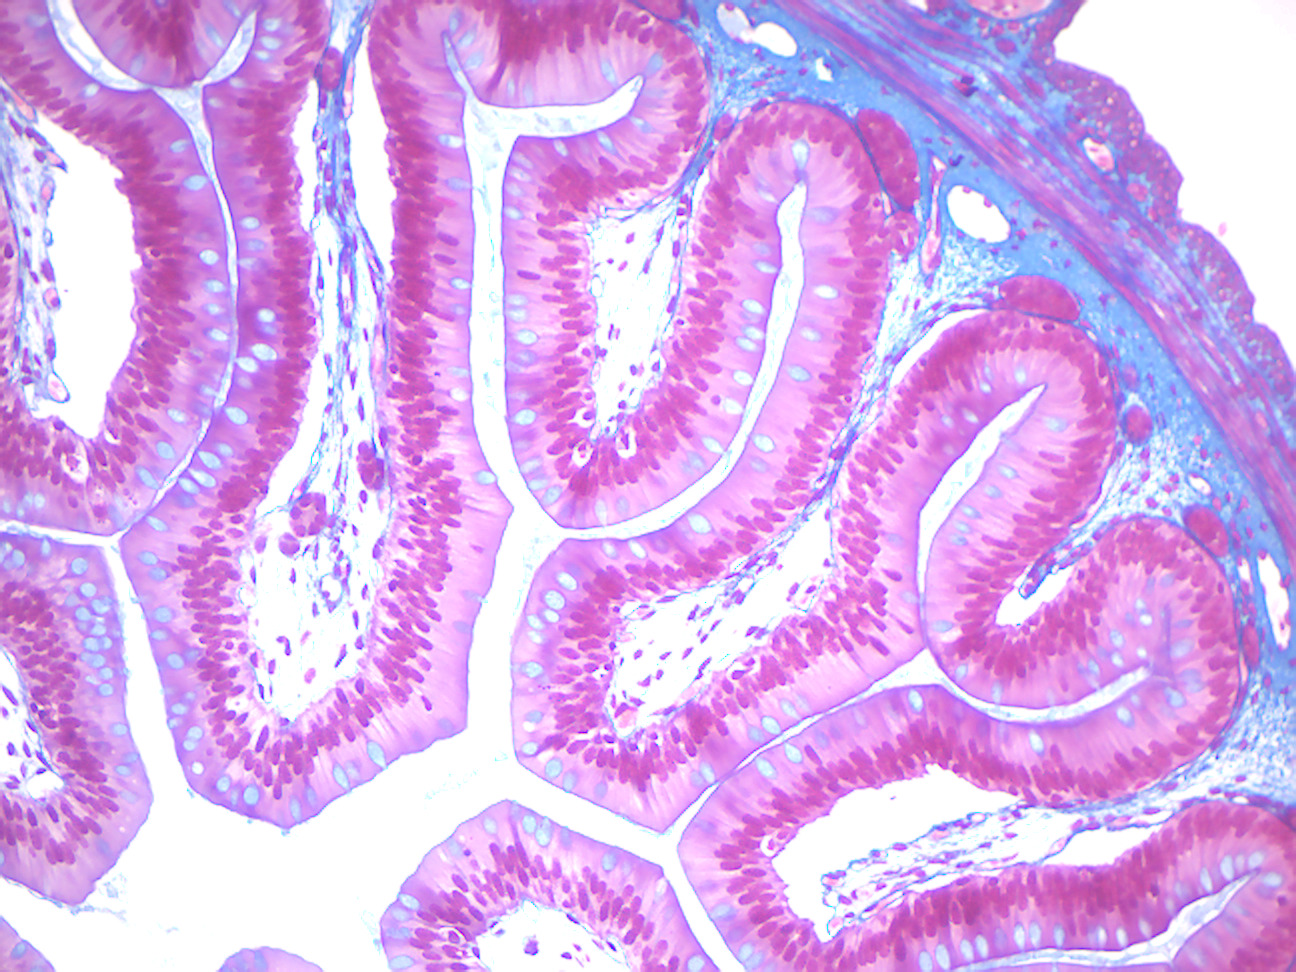
\includegraphics[width=0.7\linewidth]{./figures/tissues/simple_columnar}

}

\caption{Simple columnar epithelium (amphibian).}\label{fig:columnar}
\end{figure}

\begin{figure}

{\centering 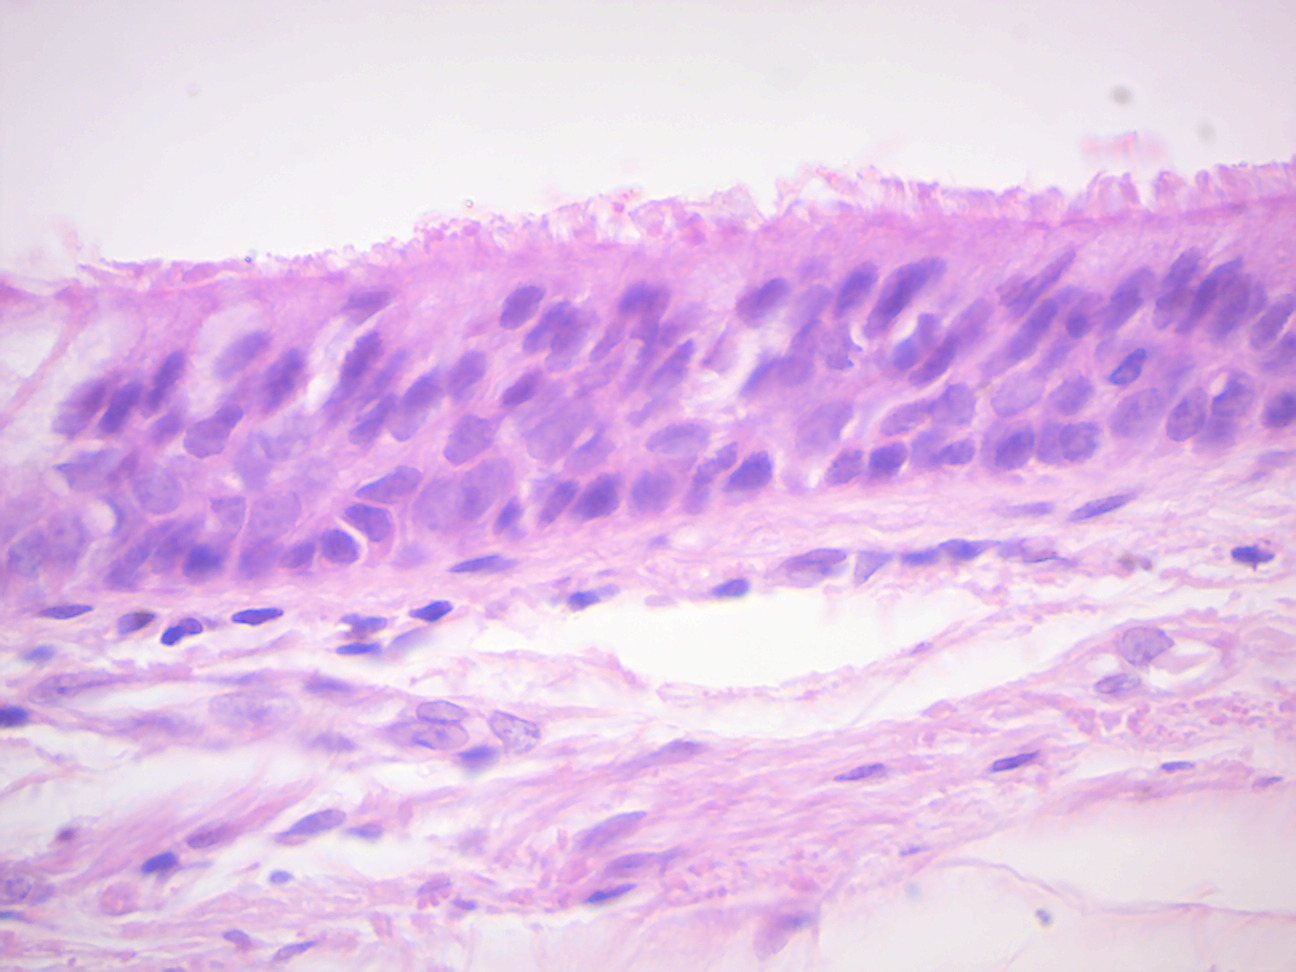
\includegraphics[width=0.7\linewidth]{./figures/tissues/pseudostratified_ciliated_columnar}

}

\caption{Pseudostratified ciliated columnar epithelium.}\label{fig:pseudociliated}
\end{figure}

\begin{figure}

{\centering 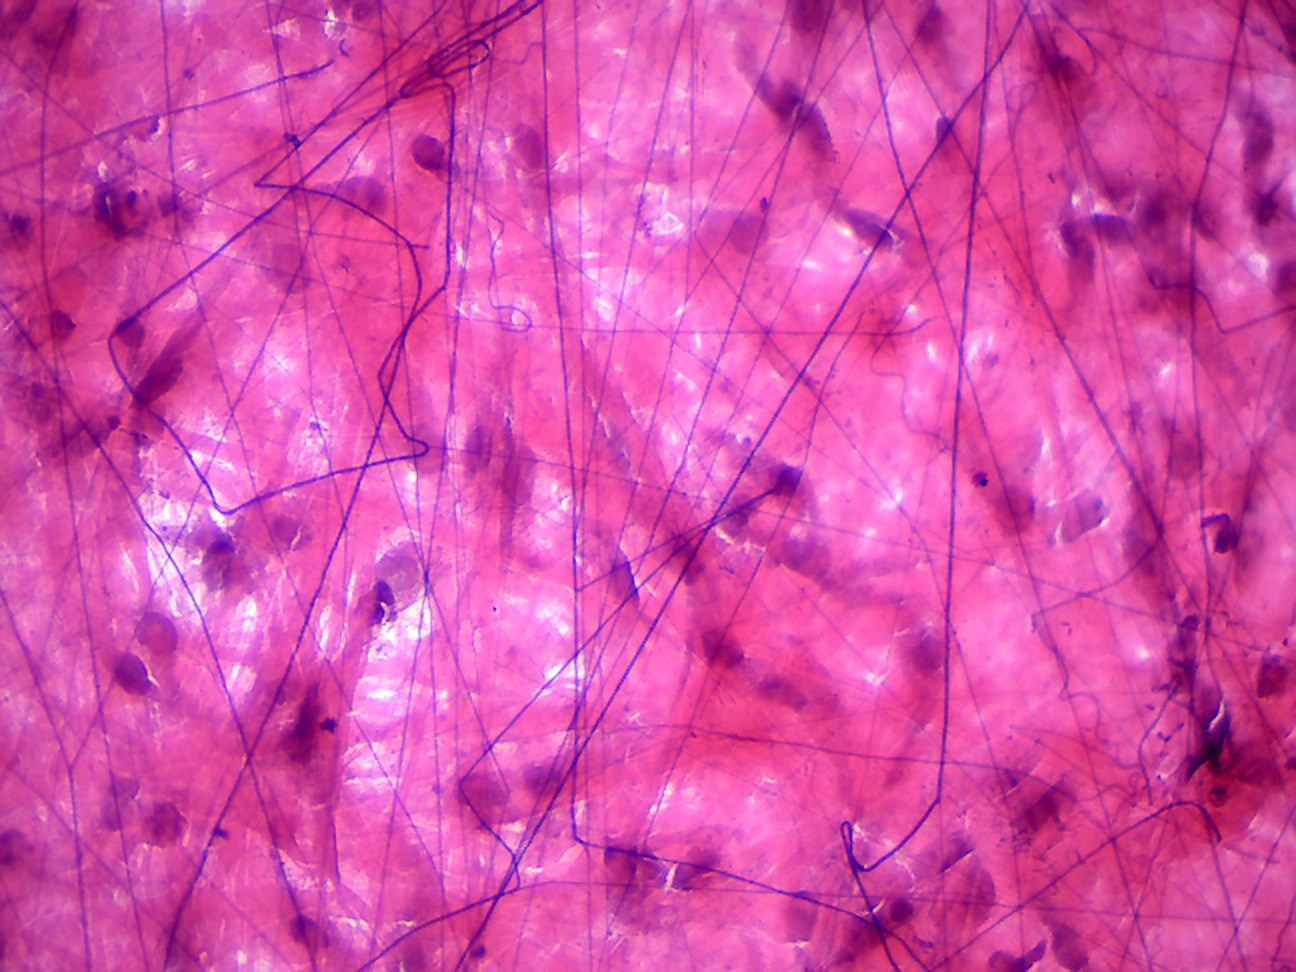
\includegraphics[width=0.7\linewidth]{./figures/tissues/areolar_spread}

}

\caption{Areolar connective tissue.}\label{fig:areolar}
\end{figure}

\begin{figure}

{\centering 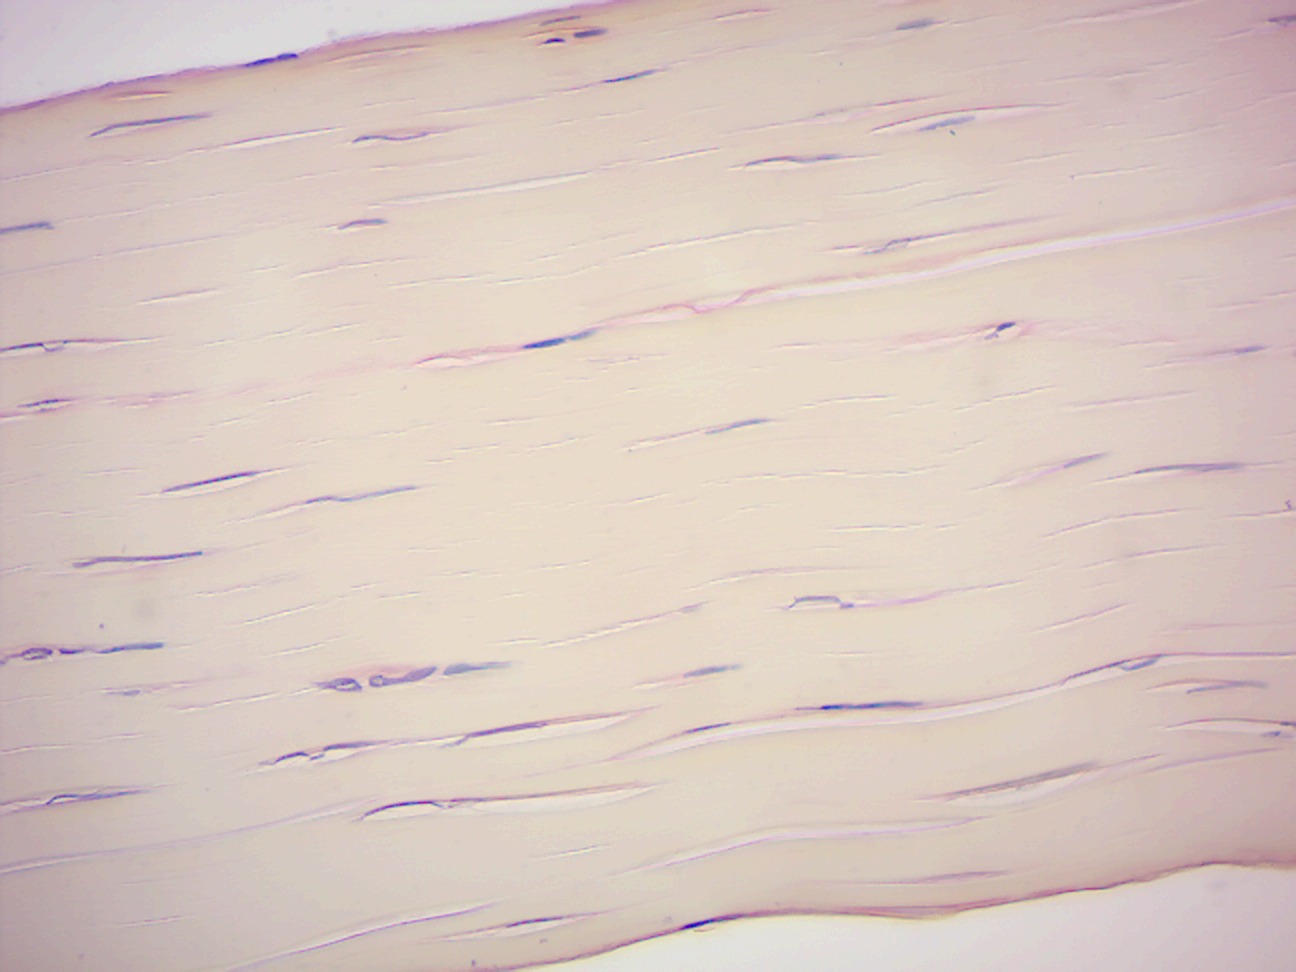
\includegraphics[width=0.7\linewidth]{./figures/tissues/white_fibrous}

}

\caption{White fibrous tissue.}\label{fig:whitefibrous}
\end{figure}

\begin{figure}

{\centering 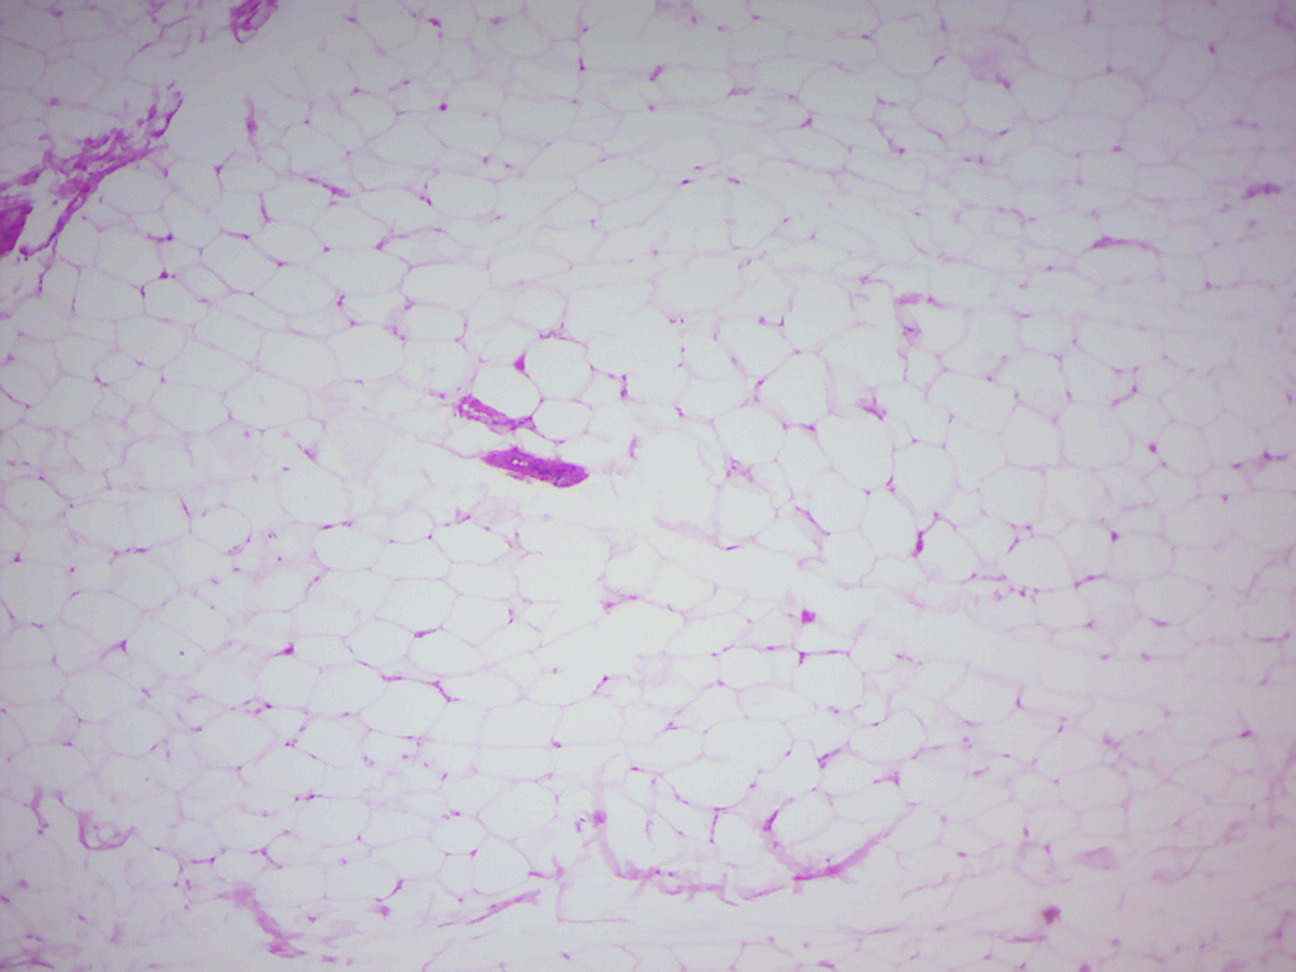
\includegraphics[width=0.7\linewidth]{./figures/tissues/adipose}

}

\caption{Adipose tissue.}\label{fig:adipose}
\end{figure}

\begin{figure}

{\centering 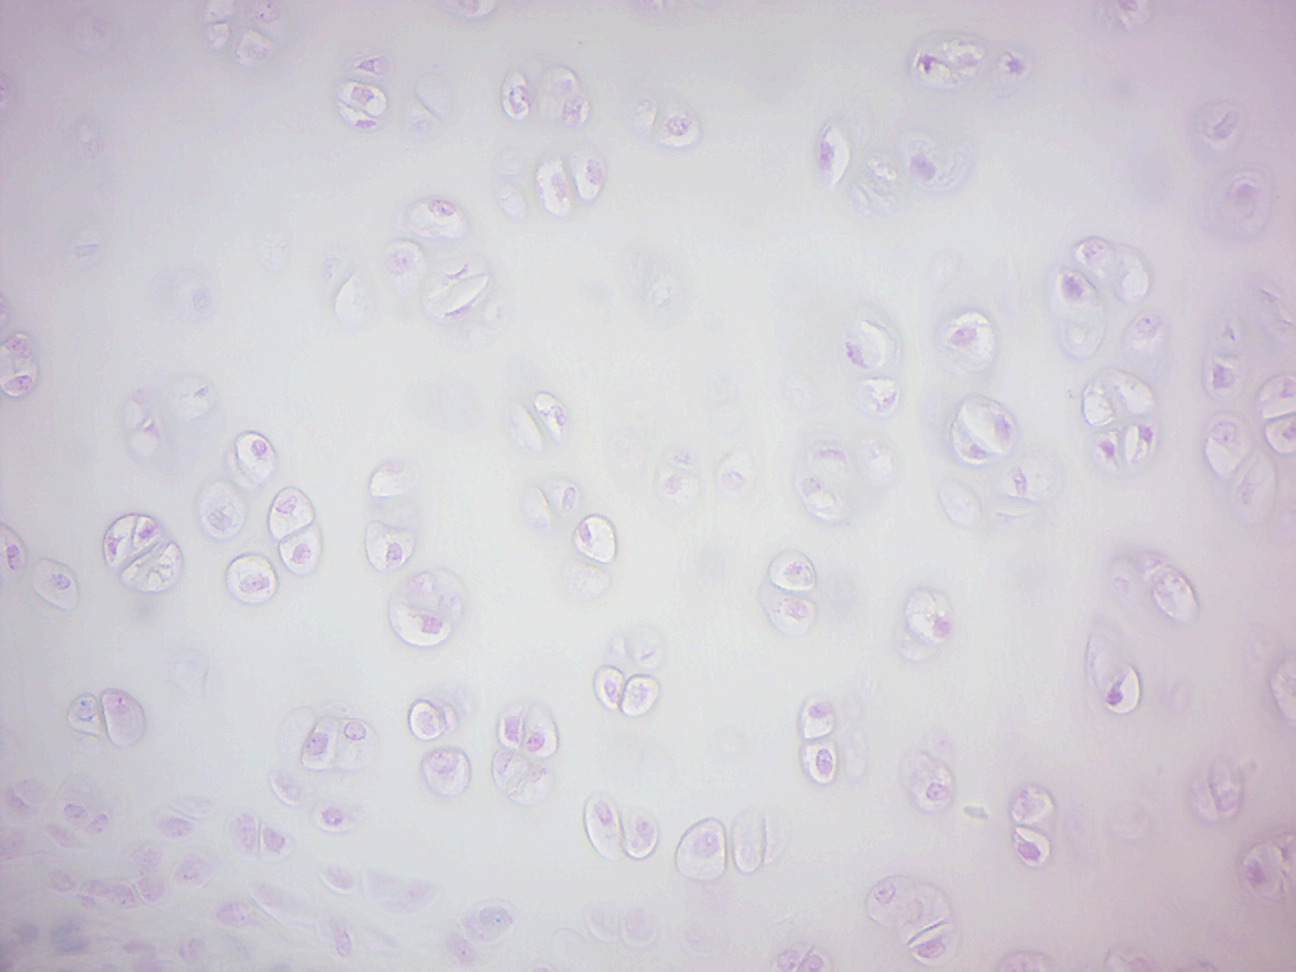
\includegraphics[width=0.7\linewidth]{./figures/tissues/hyaline_cartilage}

}

\caption{Hyaline cartilage.}\label{fig:hyaline}
\end{figure}


\begin{figure}

{\centering 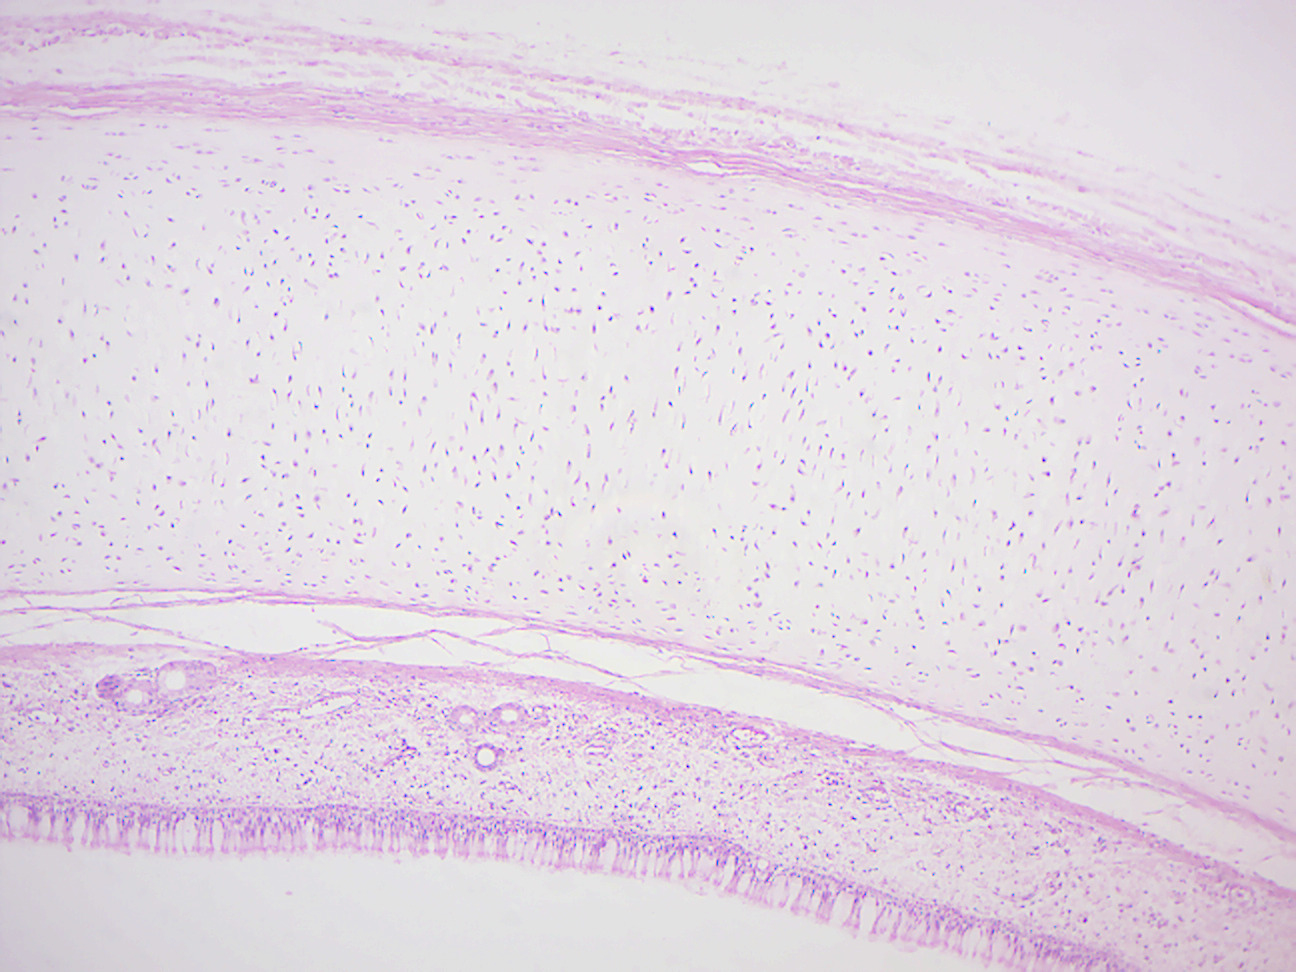
\includegraphics[width=0.7\linewidth]{./figures/tissues/monkey_trachea}

}

\caption{Monkey trachea.}\label{fig:trachea}
\end{figure}


\begin{figure}

{\centering 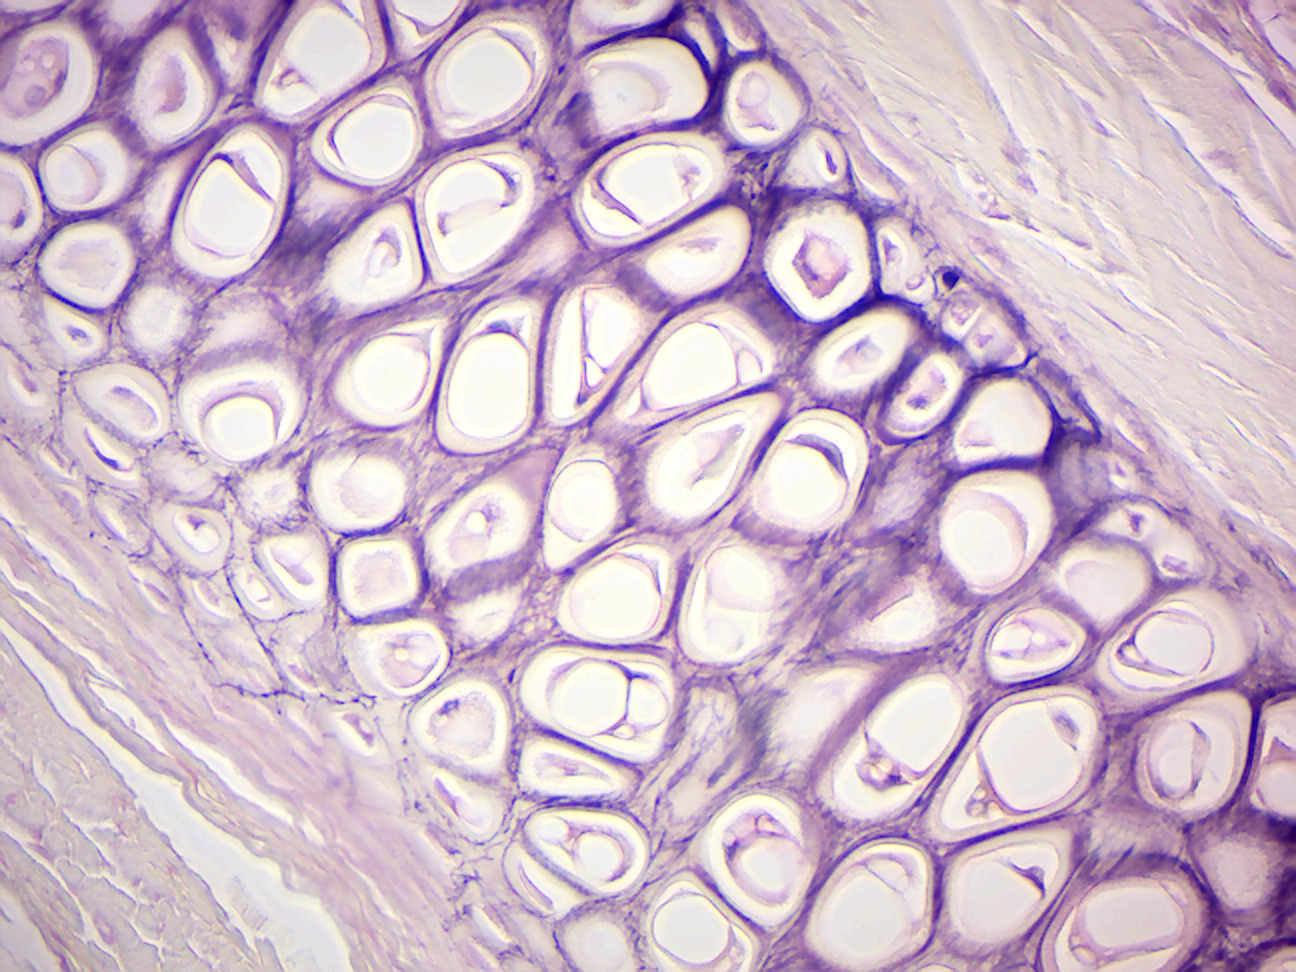
\includegraphics[width=0.7\linewidth]{./figures/tissues/elastic_cartilage}

}

\caption{Elastic cartilage.}\label{fig:elastic}
\end{figure}

\begin{figure}

{\centering 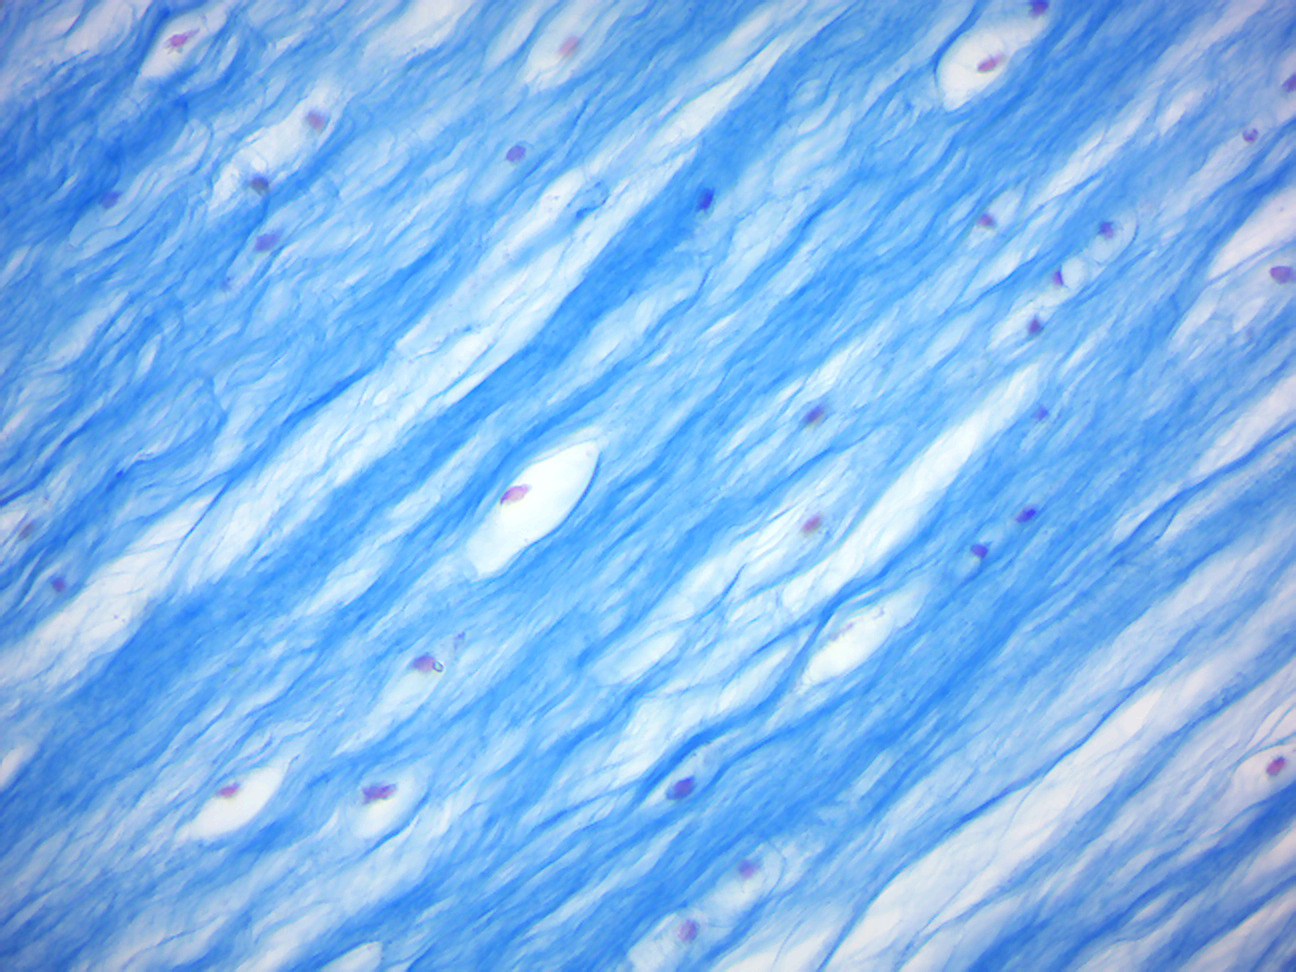
\includegraphics[width=0.7\linewidth]{./figures/tissues/fibrocartilage}

}

\caption{Fibrocartilage.}\label{fig:fibro}
\end{figure}

\begin{figure}

{\centering 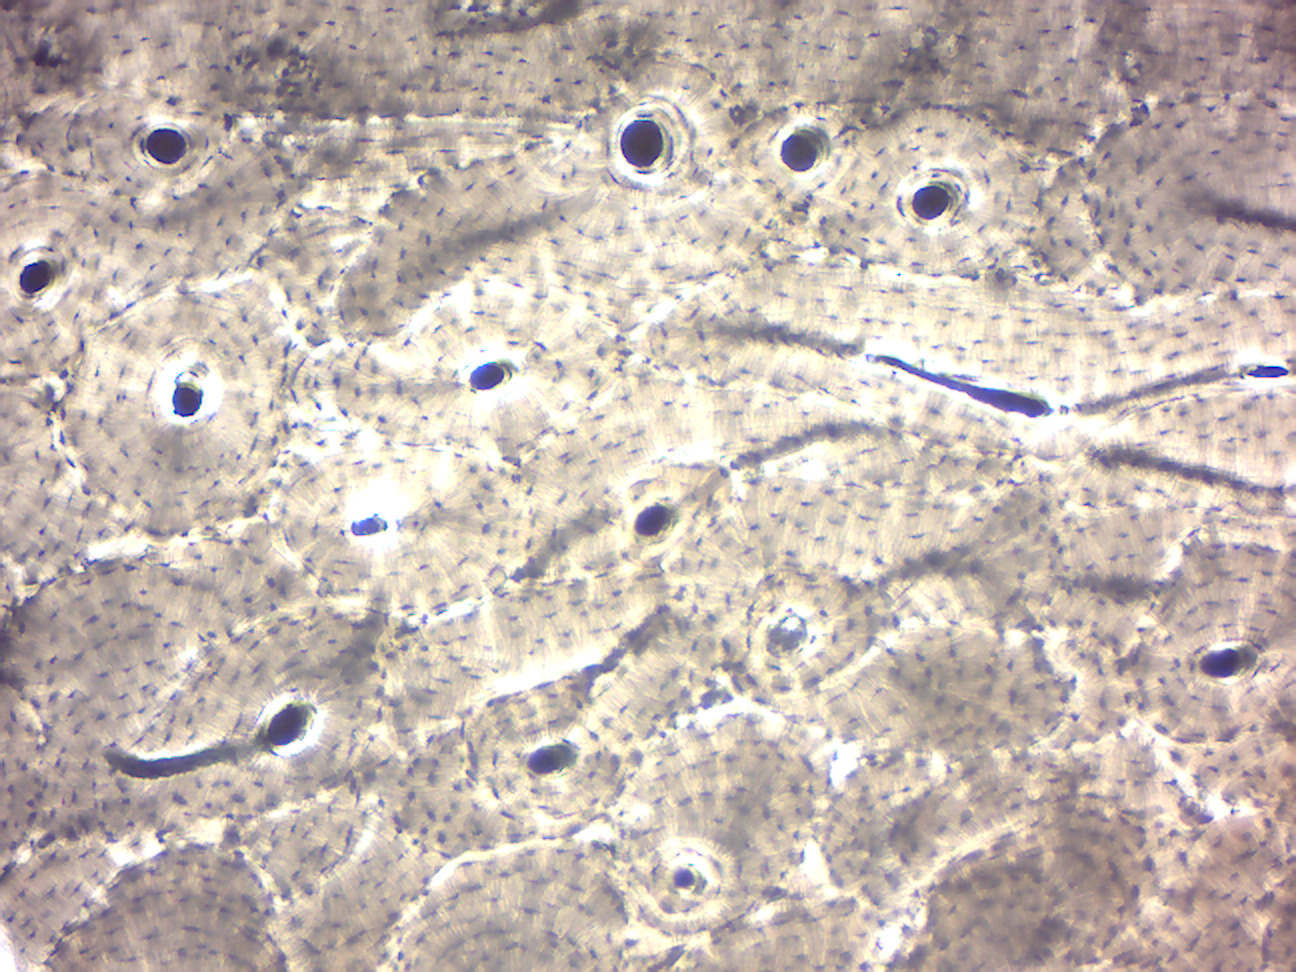
\includegraphics[width=0.7\linewidth]{./figures/tissues/ground_bone}

}

\caption{Ground bone.}\label{fig:groundbone}
\end{figure}


\begin{figure}

{\centering 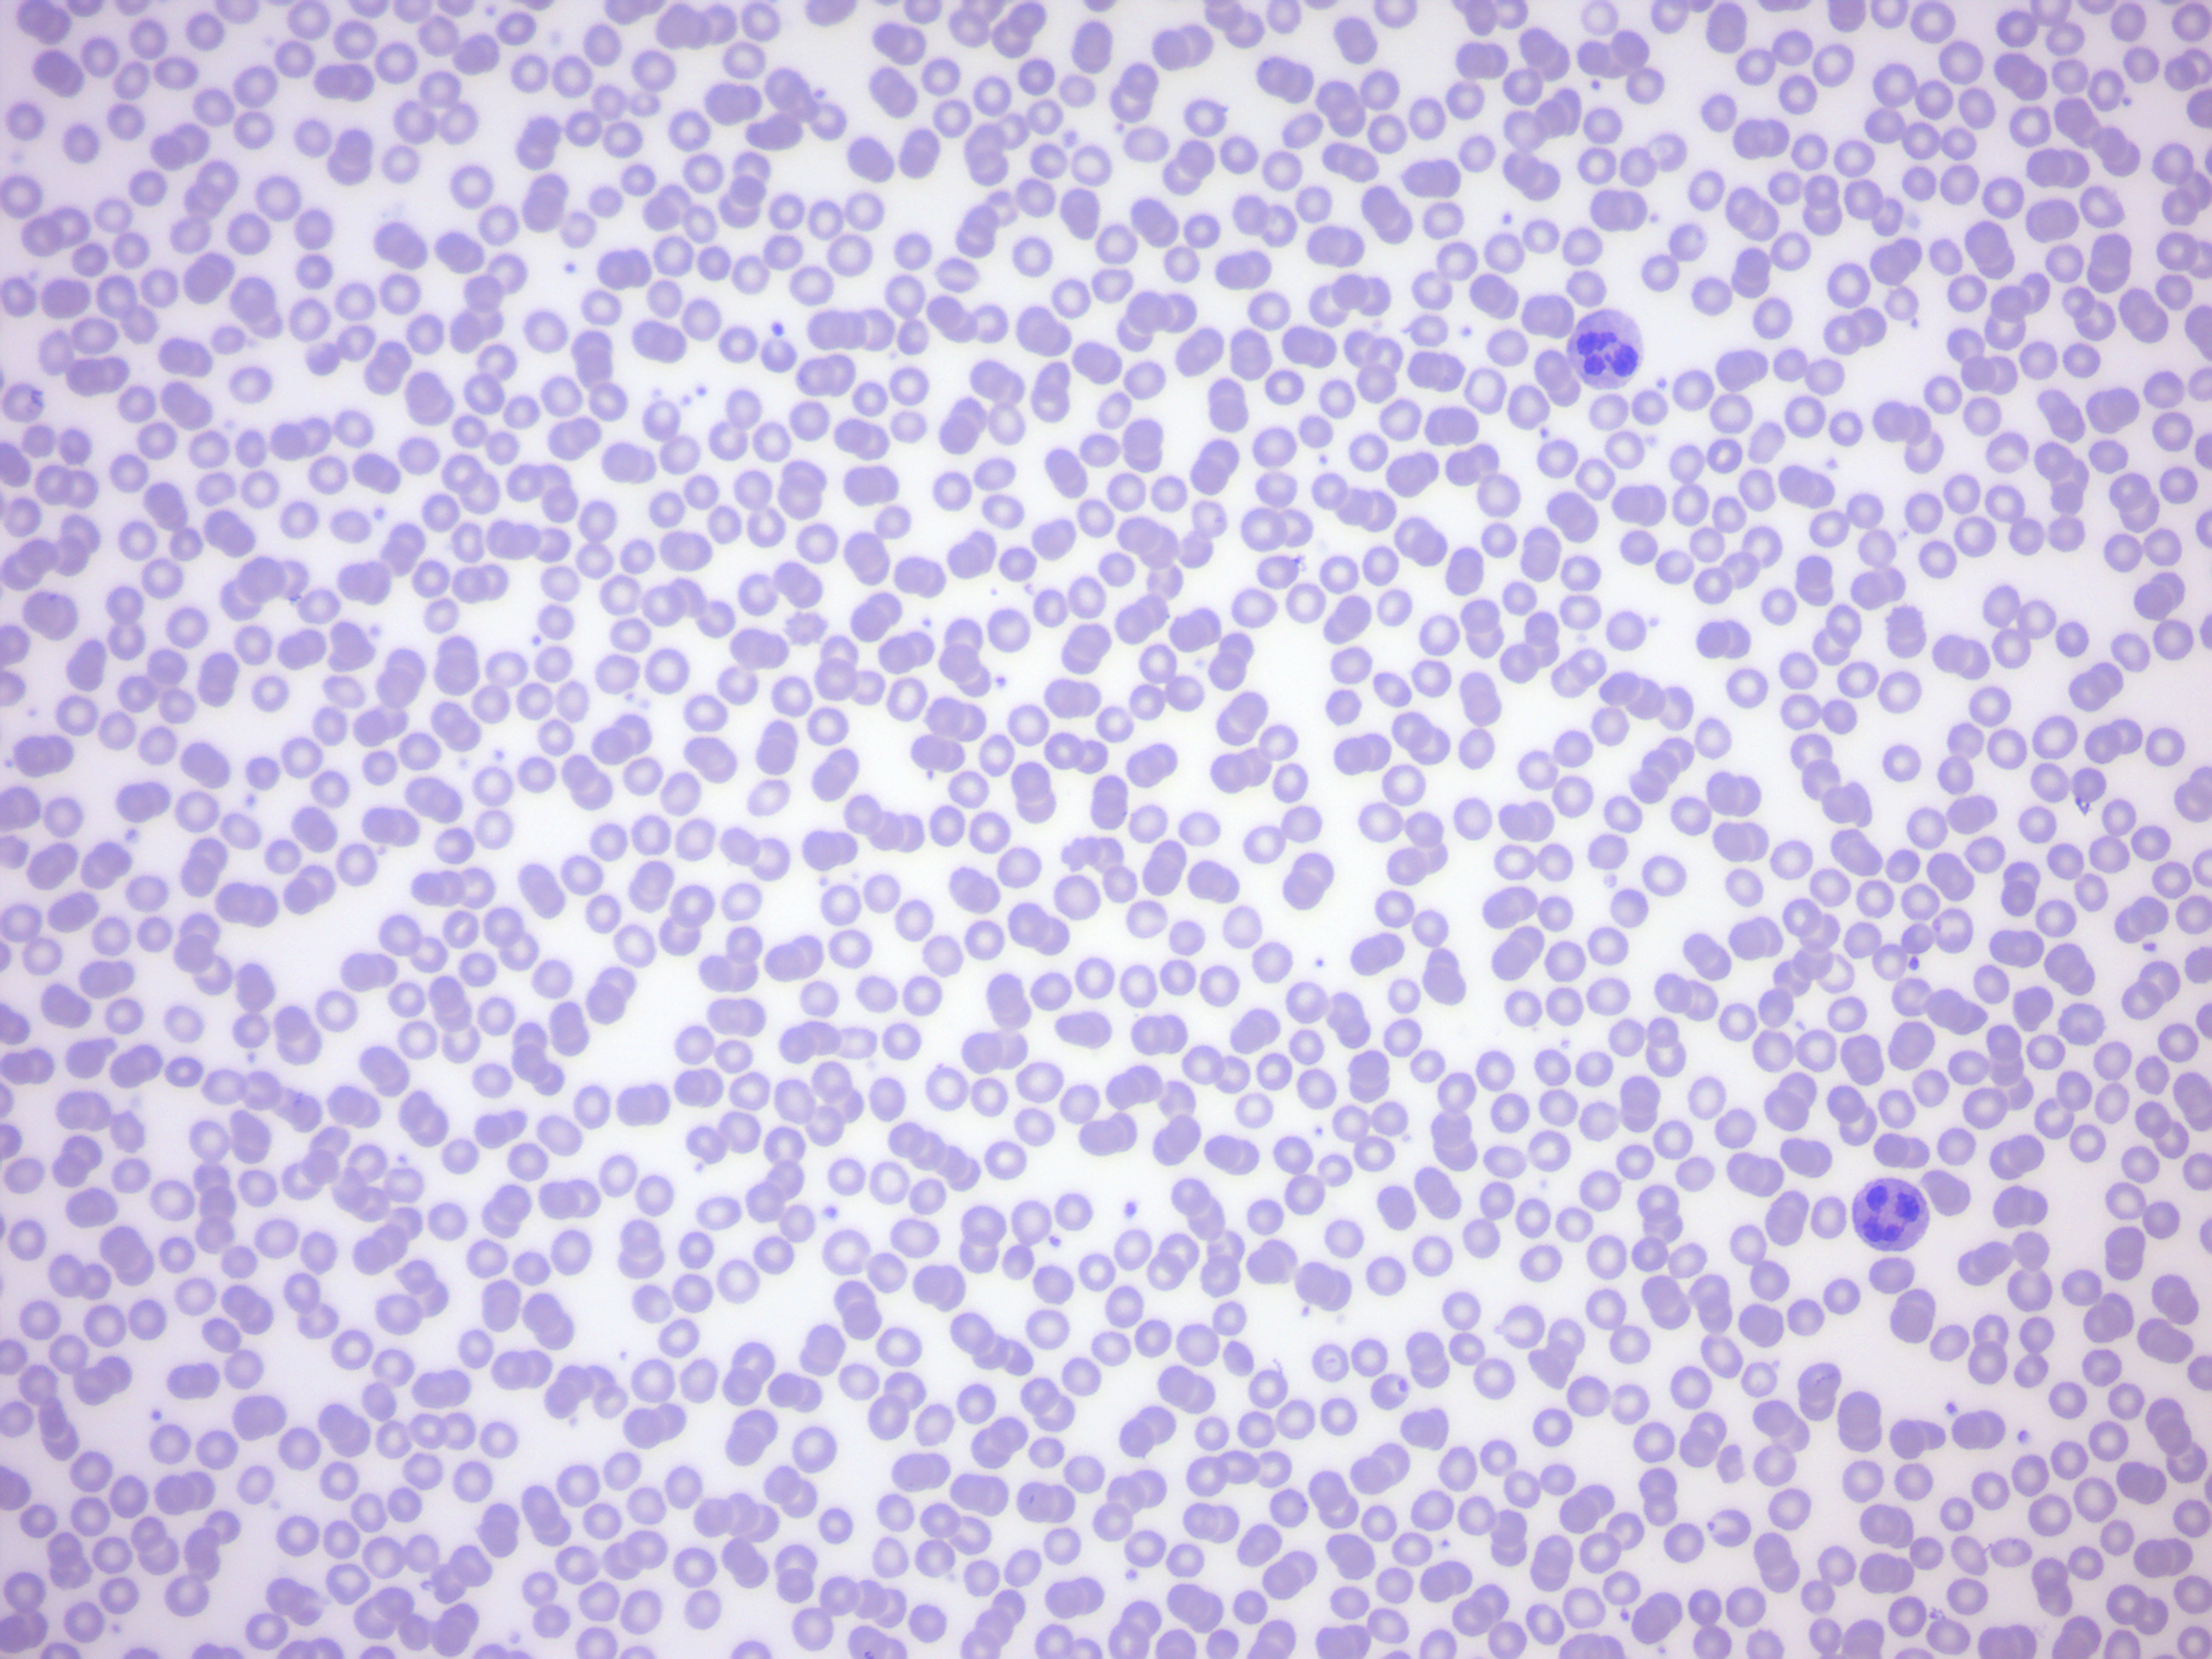
\includegraphics[width=0.7\linewidth]{./figures/tissues/blood_smear}

}

\caption{Human blood smear.}\label{fig:bloodsmear}
\end{figure}

\begin{figure}

{\centering 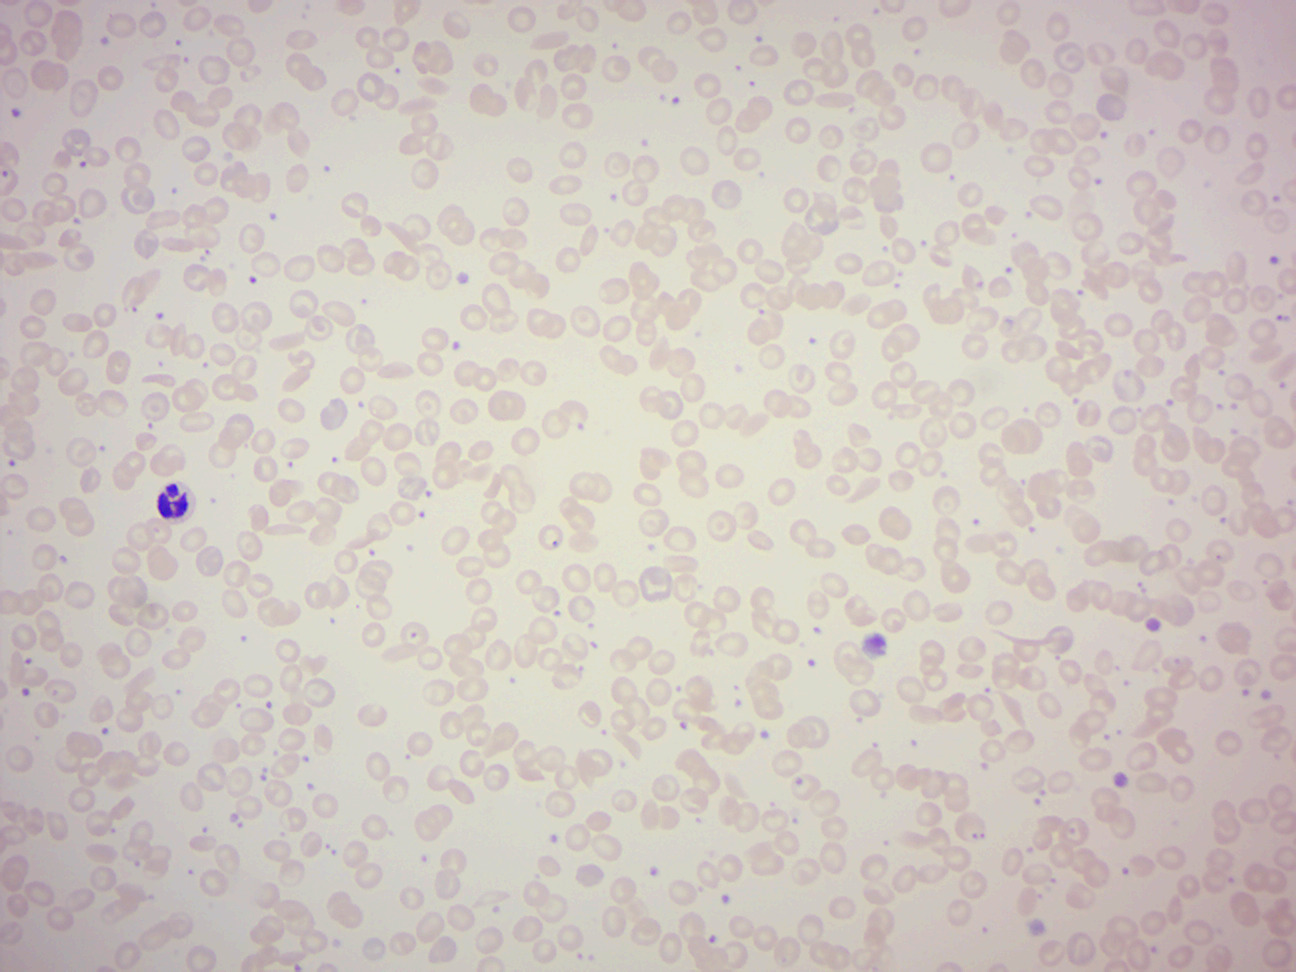
\includegraphics[width=0.7\linewidth]{./figures/tissues/sickle_cell}

}

\caption{Sickle cell blood smear.}\label{fig:sickle}
\end{figure}


\begin{figure}

{\centering 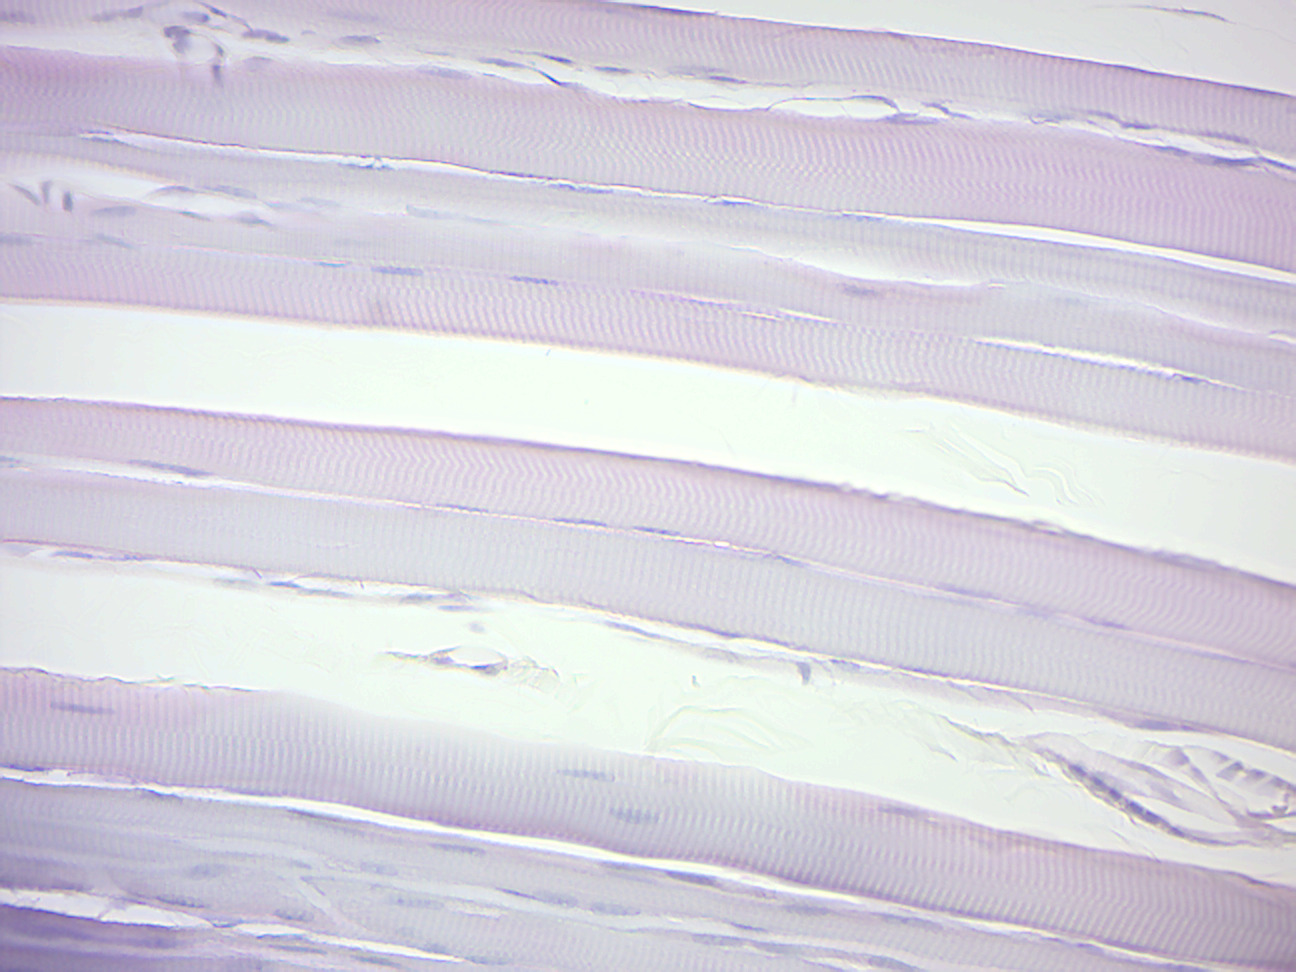
\includegraphics[width=0.7\linewidth]{./figures/tissues/skeletal_muscle}

}

\caption{Skeletal muscle.}\label{fig:skeletal}
\end{figure}

\begin{figure}

{\centering 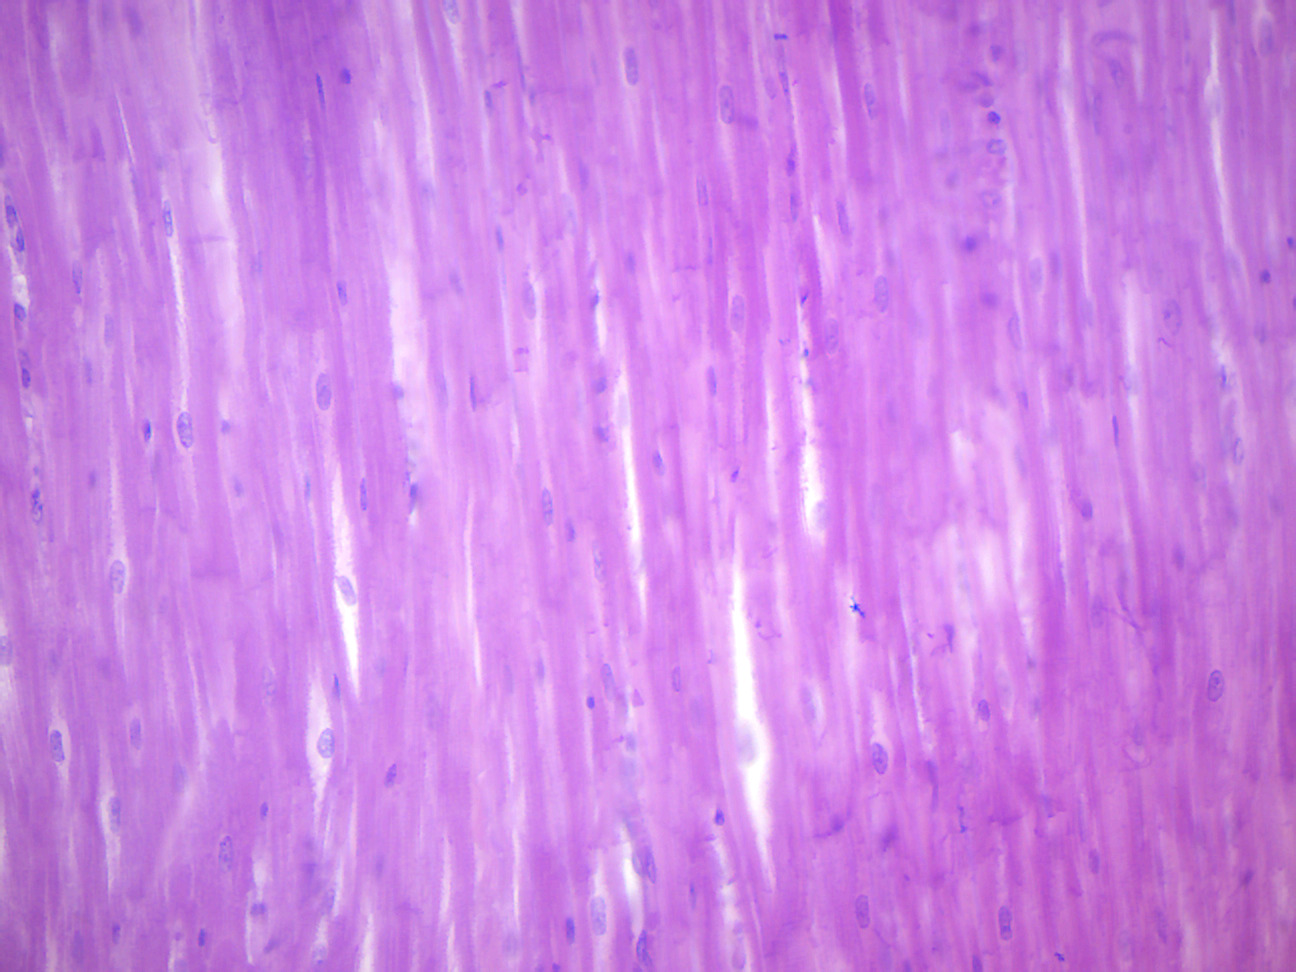
\includegraphics[width=0.7\linewidth]{./figures/tissues/cardiac_muscle}

}

\caption{Mammalian cardiac muscle.}\label{fig:cardiac}
\end{figure}




\begin{figure}

{\centering 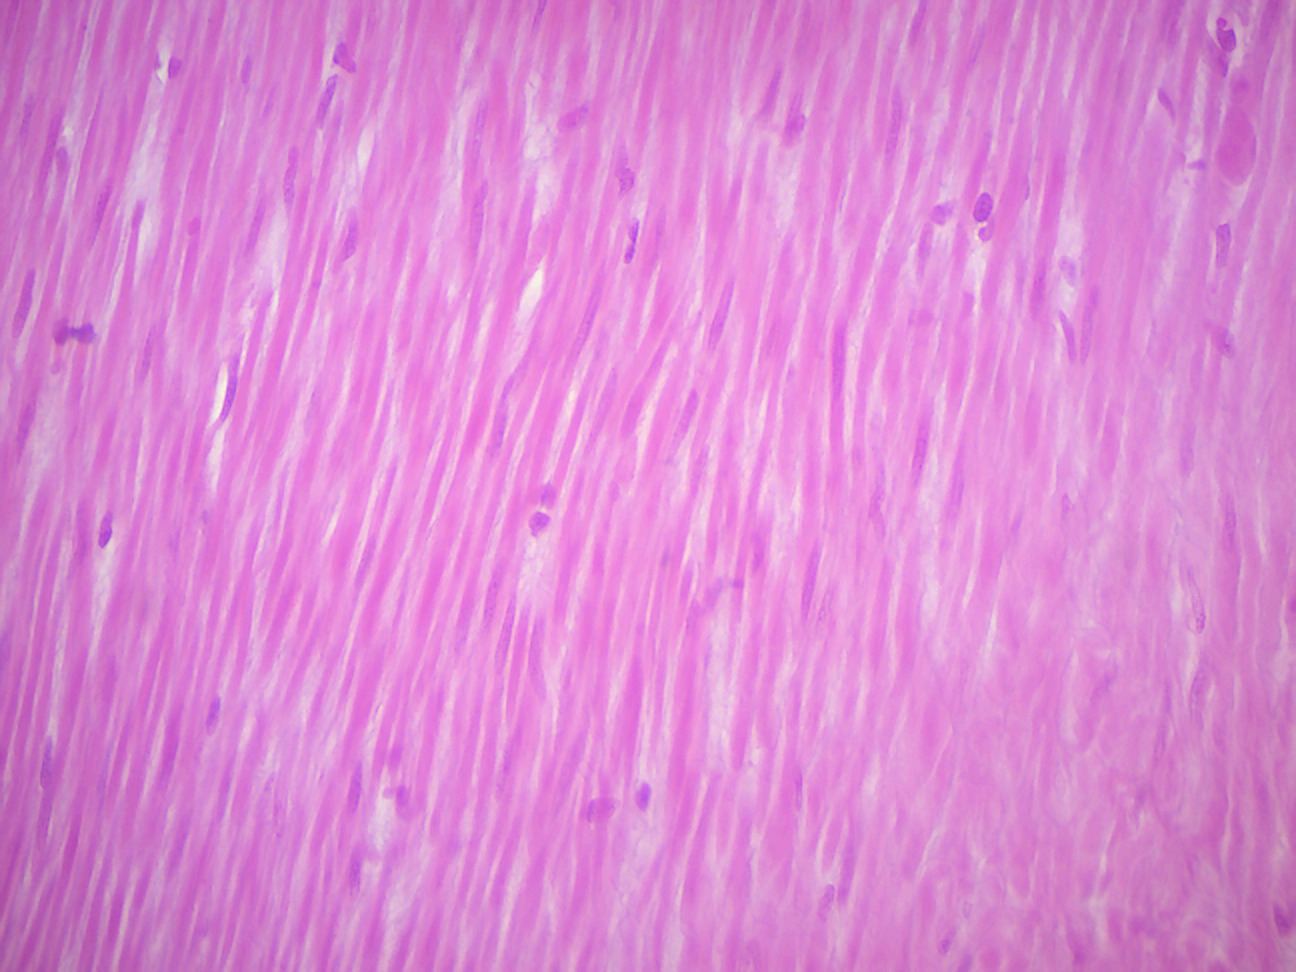
\includegraphics[width=0.7\linewidth]{./figures/tissues/smooth_muscle}

}

\caption{Smooth muscle.}\label{fig:smooth}
\end{figure}

\begin{figure}

{\centering 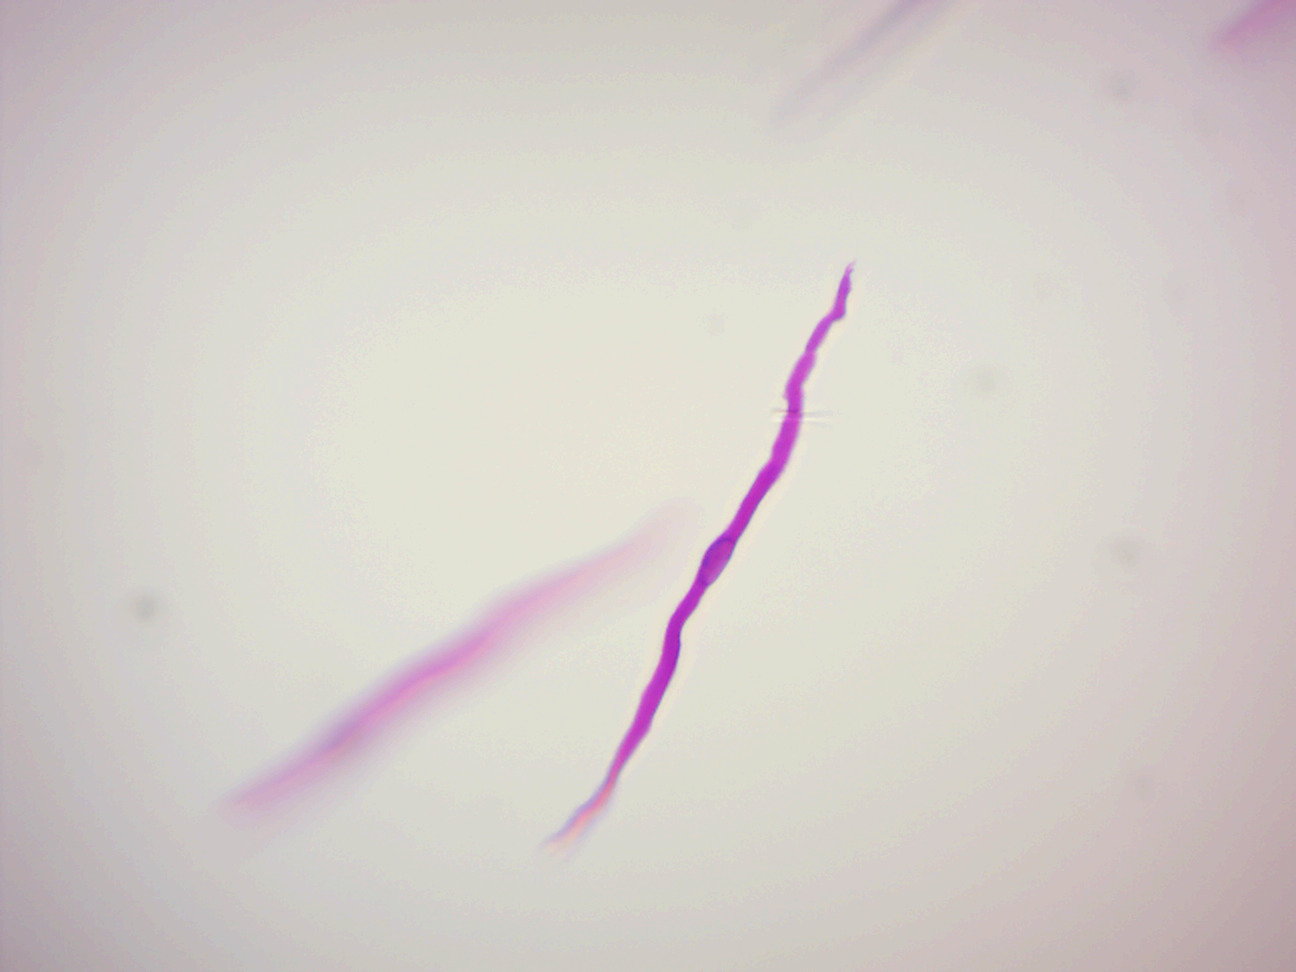
\includegraphics[width=0.7\linewidth]{./figures/tissues/smooth_muscle_teased}

}

\caption{A teased smooth muscle fiber.}\label{fig:teased}
\end{figure}

\begin{figure}

{\centering 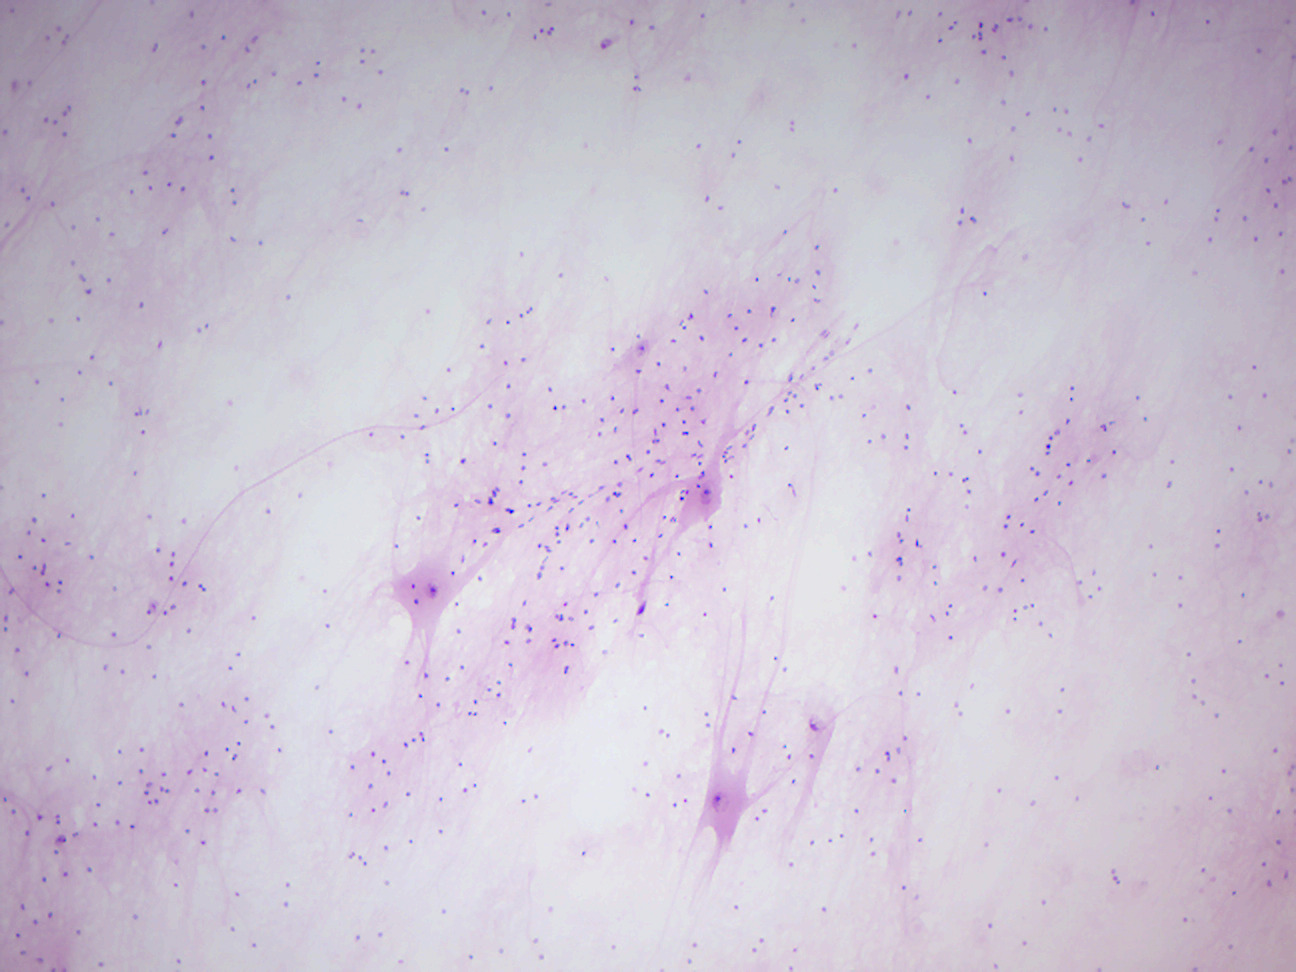
\includegraphics[width=0.7\linewidth]{./figures/tissues/neuron_smear}

}

\caption{Motor neuron smear.}\label{fig:neuron}
\end{figure}

\section{Review Questions}\label{review-questions-7}

\begin{enumerate}
\def\labelenumi{\arabic{enumi}.}
\tightlist
\item
  What are tissues?
\item
  What are the four main types of animal tissues?
\item
  What is the difference between skeletal and smooth muscle?
\item
  What is epithelial tissue?
\item
  What is connective tissue?
\item
  What are the characteristics that distinguish cardiac muscle from
  skeletal muscle?  
\end{enumerate}
